% squinch space a bit if needed
% \setlength{\parindent}{0in}
% \setlength{\parskip}{0.5ex}
\section*{Project Summary {\small (1 page)}}
\addcontentsline{toc}{section}{A. Project Summary}
%
This is a three phase project. 
The first phase is to predict the performance of a virtual disk given a workload and a storage system. 
The second phase is to model the performance interference between different virtual disks on a single storage system. 
The last phase is to map application requirements to resource mapping.

The first phase will result in virtual disk performance model. 
In our previous work with VMware, we developed a storage performance modeling framework called Romano. 
This differs from previous model, Pesto\cite{pesto}, currently in use by \emph{Virtual Center} product in that it identifies the key characteristics of workload that affects the performance (using ANOVA\cite{lilja}).
The resulting accuracy is improved by 80\% allowing much more aggressive load balancing. 
\begin{figure}[t!]
\centering
\subfloat[Pesto]{\label{rdPesto}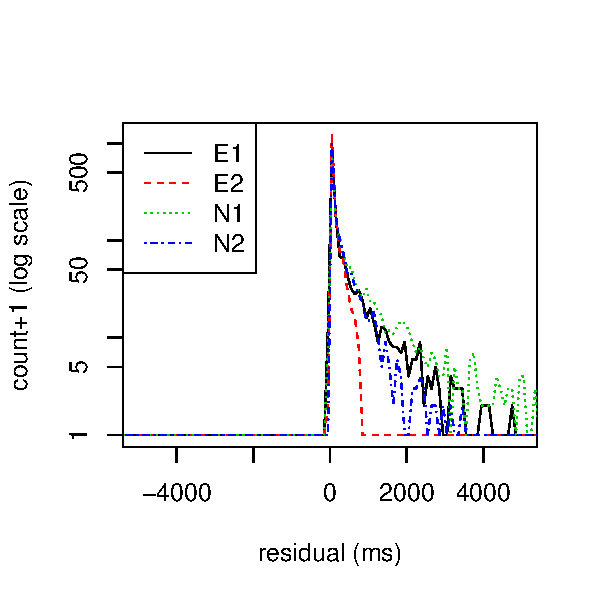
\includegraphics[width=0.4\columnwidth, clip, trim=0 0.5in 0.2in 0.7in]{error_hist_compare_pesto.pdf}}
\subfloat[Romano]{\label{rdRomano}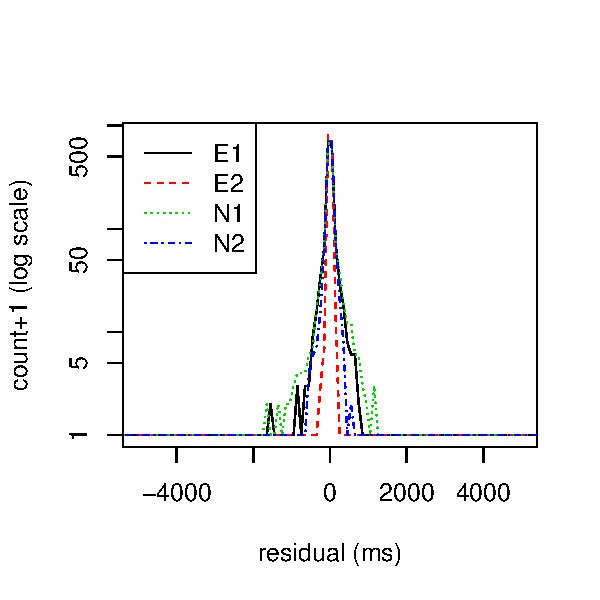
\includegraphics[width=0.4\columnwidth, clip, trim=0 0.5in 0.2in 0.7in]{error_hist_compare_kromano.pdf}}
\caption{Distribution of residuals($\epsilon$) for Pesto and Romano.
x-axis is the value of $\epsilon$ in $ms$.
y-axis is number of occurrences+1.
Addition of 1 was required to allow y-axis to be in log scale.
%The $\epsilon$ distribution does not changes widely for Romano indicating that the accuracy of Romano is less data store dependent. 
%Furthermore, Romano's $\epsilon$ are symmetric around 0, indicating that residuals are unbiased.
}
\label{residualDist}
\end{figure}
The residuals from both techniques are shown in Figure \ref{residualDist} for four different storage systems.
While this approach is very good at predicting a data store performance, it currently lacks the ability to predict the performance for each virtual disk when they are consolidated onto a single data store. 

In the second phase, we will apply statstical inference on the effect of interference, we plan to derive each VM's IO performance without having to actually change the system state.  
This allows IT administrators to simulate their configuration changes in the large scale data centers without disrupting their operation. 

The last phase will allowing application level performance requirements to be mapped to VM level configurations, users can simply specify the desired behavior without having to worry about the VMware product details.
